%From: John W Morgan <jmorgan@math.ias.edu>
%Date: Thu, 12 Jun 1997 11:07:10 -0400
%To: drm@math.ias.edu
%Subject: LEcutre II-18




\documentclass[10pt]{article}
\usepackage[dvips]{epsfig}
\usepackage{amssymb}




%sample command

%\begin{figure}
%\centerline{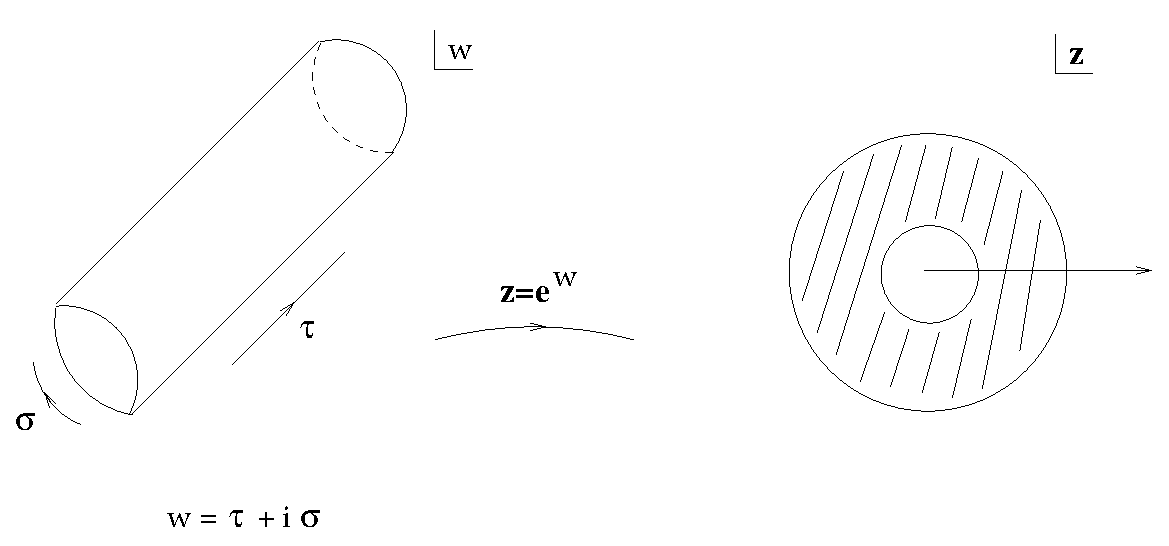
\epsfig{file=fig1.eps}}
%\end{figure}


%variant:

%\centerline{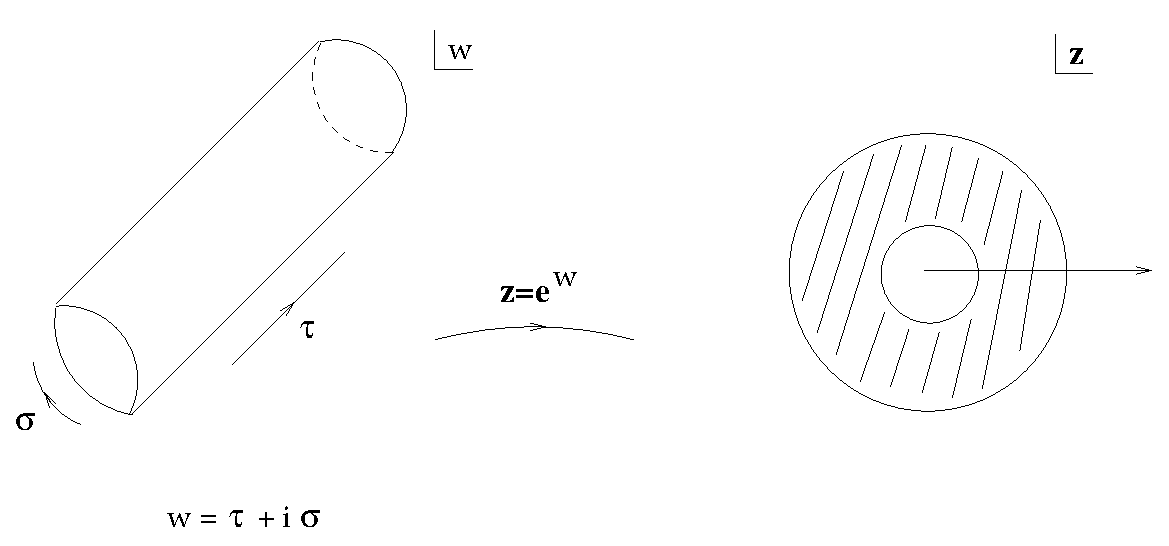
\epsfig{file=fig1.eps,height=3cm}}







%These are the macros which are in common with all of the
% sections in the paper mmr
% Each section, for now, should begin with \documentstyle[11pt,cd]{article}
% and then have \input{mmrmacros} followed by \begin{document}
% The only exception is that the \Label macro is slightly different
% in each file and should be put in separately.
%New CD macros
\newcommand{\cdrl}{\cd\rightleftarrows}
\newcommand{\cdlr}{\cd\leftrightarrows}
\newcommand{\cdr}{\cd\rightarrow}
\newcommand{\cdl}{\cd\leftarrow}
\newcommand{\cdu}{\cd\uparrow}
\newcommand{\cdd}{\cd\downarrow}
\newcommand{\cdud}{\cd\updownarrows}
\newcommand{\cddu}{\cd\downuparrows}
% (S) Proofs.
% (S-1) Head is automatically supplied by \proof.

\def\proof{\vspace{2ex}\noindent{\bf Proof.} }
\def\tproof#1{\vspace{2ex}\noindent{\bf Proof of Theorem #1.} }
\def\pproof#1{\vspace{2ex}\noindent{\bf Proof of Proposition #1.} }
\def\lproof#1{\vspace{2ex}\noindent{\bf Proof of Lemma #1.} }
\def\cproof#1{\vspace{2ex}\noindent{\bf Proof of Corollary #1.} }
\def\clproof#1{\vspace{2ex}\noindent{\bf Proof of Claim #1.} }
% End of Proof Symbol at the end of an equation must precede $$.

\def\endproof{\relax\ifmmode\expandafter\endproofmath\else
  \unskip\nobreak\hfil\penalty50\hskip.75em\hbox{}\nobreak\hfil\bull
  {\parfillskip=0pt \finalhyphendemerits=0 \bigbreak}\fi}
\def\endproofmath$${\eqno\bull$$\bigbreak}
\def\bull{\vbox{\hrule\hbox{\vrule\kern3pt\vbox{\kern6pt}\kern3pt\vrule}\hrule}}
\addtolength{\textwidth}{1in}                  % Margin-setting commands
\addtolength{\oddsidemargin}{-.5in}
\addtolength{\evensidemargin}{.5in}
\addtolength{\textheight}{.5in}
\addtolength{\topmargin}{-.3in}
\addtolength{\marginparwidth}{-.32in}
\renewcommand{\baselinestretch}{1.6}
\def\hu#1#2#3{\hbox{$H^{#1}(#2;{\bf #3})$}}          % #1-Cohomology of #2
\def\hl#1#2#3{\hbox{$H_{#1}(#2;{\bf #3})$}}          % #1-Homology of #2
\def\md#1{\ifmmode{\cal M}_\delta(#1)\else  % moduli space, delta decay of #1
{${\cal M}_\delta(#1)$}\fi}
\def\mb#1{\ifmmode{\cal M}_\delta^0(#1)\else  %moduli space, based, delta
					      %decay of #1
{${\cal M}_\delta^0(#1)$}\fi}
\def\mdc#1#2{\ifmmode{\cal M}_{\delta,#1}(#2)\else    %moduli space, delta
						      %decay, chern class #1
						      %of #2
{${\cal M}_{\delta,#1}(#2)$}\fi}
\def\mbc#1#2{\ifmmode{\cal M}_{\delta,#1}^0(#2)\else   %as before, based
{${\cal M}_{\delta,#1}^0(#2)$}\fi}
\def\mm{\ifmmode{\cal M}\else {${\cal M}$}\fi}
\def\ad{{\rm ad}}
\def\msigma{\ifmmode{\cal M}^\sigma\else {${\cal M}^\sigma$}\fi}
\def\cancel#1#2{\ooalign{$\hfil#1\mkern1mu/\hfil$\crcr$#1#2$}}
\def\dirac{\mathpalette\cancel\partial}
\newtheorem{thm}{Theorem}
\newtheorem{theorem}{Theorem}[subsection]
\newtheorem{proposition}[theorem]{Proposition}
\newtheorem{lemma}[theorem]{Lemma}
\newtheorem{claim}[theorem]{Claim}
\newtheorem{example}[theorem]{Example}
\newtheorem{corollary}[theorem]{Corollary}
\newtheorem{D}[theorem]{Definition}
\newenvironment{defn}{\begin{D} \rm }{\end{D}}
\newtheorem{addendum}[theorem]{Addendum}
\newtheorem{R}[theorem]{Remark}
\newenvironment{remark}{\begin{R}\rm }{\end{R}}
\newcommand{\note}[1]{\marginpar{\scriptsize #1 }} 
\newenvironment{comments}{\smallskip\noindent{\bf Comments:}\begin{enumerate}}{\end{enumerate}\smallskip}

\renewcommand{\thesection}{\Roman{section}}
\def\eqlabel#1{\addtocounter{theorem}{1}
\write1{\string\newlabel{#1}{{\thetheorem}{\thepage}}}
\leqno(\rm\thetheorem)}
\def\cS{{\cal S}}
\def\ov{\overline}













\title{Lecture II-18: $N=2$ Super-symmetric Yang-Mills theories in
dimension four: Part II}  
\author{Edward Witten\thanks{Notes by John Morgan}}
\date{}
\begin{document}
\maketitle


\section{Review of material from the last lecture}

We are considering pure $N=2$
super-symmetric gauge theory (i.e.,  
without hyper-multiplets) in four-dimensional Minkowski space.  The
gauge group is either $SU(2)$ or the 
closely related group $SO(3)$. 
(In fact, working as we are today over Minkowski four-space, which is
contractible, we 
will not see the distinction between these two gauge groups.)
We write the theory in the $N=1$
super-symmetric notation. The fields which form a single $N=2$ vector
multiplet decompose under the $N=1$ super Poincar\'e group in four
dimensions as a vector  
multiplet ${\cal A}$ (the gauge fields) and a chiral super-field
$$\Phi=\phi+\theta\psi+\cdots$$
where $\phi$ is a scalar field (under the Poincar\'e group).
It is a section of the complexification of the adjoint bundle.
The microscopic Lagrangian is
$${\cal L}=\int d^4xd^2\theta\tau_0(\Lambda_0){\rm
Tr}W_\alpha W^\alpha+{\rm c.c.} +\int d^4xd^2\theta {\rm
Im}\tau_0(\Lambda_0) {\rm Tr}(\overline\Phi\Phi)$$
where $W$ is a certain piece of the super-connection of the
super-connection ${\cal A}$. 
(Here $\Lambda_0$ is a cut-off used to render finite the Feynmann path
integrals. We  vary $\tau_0$ as a function of $\Lambda_0$ in
order to renormalize, i.e., render the expectation values in the
theory finite as $\Lambda_0\mapsto\infty$. In order to decide how to
renormalize we must fix a 
so-called `subtraction point' $\Lambda$ at which to fix the value of
one parameter in the theory.  We shall see later a convenient
normalization scheme for this particular theory which involves the
details of the theory (the $u$-plane, etc).  But for now we leave
vague the actual renormalization scheme. Once we have fixed the value
of the extra parameter $\Lambda$, the coupling constant $\tau_0$
is a function of $\Lambda_0$.)   While $\tau$ depends
on the cut-off, it is 
independent of the fields. 

Our object today is to solve this theory by
explicitly understanding the moduli space ${\cal M}$ of quantum vacua,
as well as a description of the theory near each vacuum state.
As we established last time, the space of classical vacua of this
theory consists of
gauge equivalence classes of constant matrices in $su(2)$
$$\frac{1}{\sqrt{2}}\pmatrix{a & 0 \cr 0 & -a}$$
modulo the action of the Weyl group, which is a group of order two
switching $a$ and $-a$. This space is analytically isomorphic to ${\bf
C}$ and the natural local holomorphic coordinate to use on this plane
is $u={\rm Tr} \phi^2=a^2$. While the analytic space of classical vacua is
smooth, there is one point in the moduli
space of classical vacua where the K\"ahler metric becomes singular.
This is the origin. The singularity is a consequence of the fact that
at this point there are more
massless fields (in fact a super-symmetric $SU(2)$-theory is the lower
energy effective theory). Furthermore, as we discussed last time,
away from $u=0$ the low energy effective theory is a pure $N=1$
super-symmetric $U(1)$-gauge theory.
Thus, away from $u=0$, the
nature of this effective theory is described by a family of tori over the
punctured $u$-plane.  In the case of the moduli space of classical
vacua this is a family of tori with constant $j$ invariant
given by the choice of $\tau$ in the Lagrangian.  The monodromy around
infinity for this family is $-1$.  The K\"ahler metric on the
$u$-plane is
$$ds^2={\rm Im}\tau\frac{du d\overline{u}}{4|u|^2}.$$
(Notice that there is a singularity in the metric at $u=0$ as
predicted by the fact that at this vacuum there are extra massless
fields classically.)



\subsection{First results about the moduli space ${\cal M}$ of quantum
vacua} 


Let ${\cal M}$ be the space of quantum vacua.
Notice that, because we are assuming that our theory is $N=2$
super-symmetric, the space of quantum vacua has a K\"ahler metric (from
the weaker $N=1$ super-symmetry) and over this space of vacua there is
a holomorphic family of tori. The field $u$, which is a coordinate on
the space of classical vacua, 
 is a chiral field in the
theory, and thus its expectation 
values in the various quantum vacua defines a holomorphic
function on  ${\cal M}$.
We denote this function by $u\colon {\cal M}\to {\bf C}$:
$$u(\Omega)=\langle \Omega|u|\Omega\rangle, \ \ \ {\rm for\ all}\
\Omega\in{\cal M}.$$ 



The part of ${\cal M}$ that is most closely related to the $u$-plane
of classical vacua is the region where $u$ is large.
More precisely, suppose that we have fixed  the mass parameter,
$\Lambda$, in
the renormalization scheme which determines the specific quantum
theory  we are studying. Suppose that we are studying the theory near
a classical vacuum $\Omega$ with $u(\Omega)>> \Lambda^2$. (Notice that
since $u$ has dimensions of mass squared it naturally compares to
$\Lambda^2$.) Because our $SU(2)$-theory is asymptotically free, and
the $U(1)$-theory to which it is limiting is free in the infra-red, if
$u>>\Lambda^2$, then the quantum theory is well-approximated near 
$\Omega$ by the classical theory.  This means that the low energy
quantum theory near $\Omega$ is described by a sigma model on the
$u$-plane, perhaps perturbed by some super-potential. 
But $N=2$  super-symmetry means that any
such super-potential must be a constant, and hence cannot lift the
vacuum degeneracy near $\Omega$.  (There is also the possibility of a
Fayet-Iliopoulos $\theta$-term  to consider as well, but the
$SU(2)_R$-symmetry rules these out.)  What this argument shows is that
for large $u$ there is a unique quantum vacuum for
each classical vacuum.
That is to say, there is a constant $C(\Lambda)>0$ and an open subset
${\cal U}\subset {\cal M}$ with the property that $u\colon {\cal U}\to 
(\{z\in {\bf C}| |z|>C\})$ is a holomorphic
isomorphism.


In Seiberg's lectures we have seen other examples of gauge theories
where near infinity in 
the space of classical vacua the
gauge group $SU(N_c)$ is broken down to a non-abelian gauge group
$SU(N_c-N_f)$. Since the gauge theory for this smaller group is not
free in the infra-red, we cannot conclude that the space of
quantum vacua near infinity can be identified with the subspace of
critical points of a superpotential on the space of classical vacua.
In fact, in
these examples the moduli space of quantum vacua is a finite covering
space of the space of classical vacua near infinity.  To repeat, this
is possible because the low energy theory is not free in the
infra-red.  When it is free, as in the case under discussion now, and
when $N=2$ super-symmetry rules out the existence of super-potentials, the
classical and quantum moduli spaces can be identified over a
neighborhood of infinity in the space of classical vacua.


One assumption that we shall make without any justification is that
the moduli space ${\cal M}$ is
complete in an appropriate sense so that it corresponds to an open
complex algebraic variety.






We have found one component of ${\cal M}$ which has an end
isomorphic under $u$ to a neighborhood of infinity in 
${\bf C}$.
Two other questions present themselves:
\begin{itemize}
\item Are there other `ends' of ${\cal M}$, ends that are not seen
classically?
\item Are there other irreducible components of ${\cal M}$ not seen
classically?  
\end{itemize}

The answer to the first question is `No.' The point is that all ends
of the quantum moduli space must be visible classically, i.e, they
must be related to ends of the classical moduli space.  The reason is
that quantum effects are bounded and hence cannot effect a non-proper
change in the passage from the space of classical vacua to the space
of quantum vacua.

As to the second question,
there are no examples known 
where there are branches of the quantum space of vacua which are not
seen classically.  Still in this generality, it has not been
established that such components do not exist.  Nevertheless, in our
case we can give arguments  showing
that there are no other components.
The first thing to note is that, by the answer to the first question,
any other component of ${\cal M}$ must 
be compact. 
To exclude the possibility of other compact branches we use the fact
that the theory has a relevant $N=1$ super-symmetric perturbation.
That is the perturbation
$$\Delta{\cal L}=\int d^4xd^2\theta \epsilon u+{\rm c.c.}$$
where $\epsilon$ is a complex constant.
As we saw in Lecture II-??, with this perturbation the resulting
$SU(2)$-theory 
has two vacua, each with a mass gap and each with confinement.
If we examine  what happens to these perturbed theories in the low energy
limit, then of course they look the same: they have two vacua each
with a mass gap and confinement.  Thus, this perturbation would have to lift
the vacuum degeneracy along a compact 
component ${\cal N}$ of ${\cal M}$ by adding a super-potential.
On the other hand, since $u$ is a holomorphic function along this
branch, it is constant. Now the super-potential term that we have added
to the microscopic Lagrangian is simply $\epsilon u$ which is constant
along this branch. One can see that this persists in the low energy
theory, so that the low energy effective super potential is also a
multiple of $u$, and hence is constant.  This means that the addition
of the above super-potential cannot lift the vacuum degeneracy along
this branch.  Since we  know the resulting low energy theory has only
two vacua, this implies that the other branch is in fact not present.
(This argument still allows for the possibility of isolated points (at
most two), but we shall see later by counting singularities, that they do
not occur either.) 

We  have now argued that ${\cal M}$ has a single branch (plus possibly
at most two isolated points) and that this
branch has a single neighborhood of infinity which is mapped by $u$
isomorphically to a neighborhood of infinity in the $u$-plane.
By our completeness assumption, we know that ${\cal M}$ is a possibly
singular, irreducible complex curve with one puncture.
The existence of the holomorphic function $u$ with a only one pole,
that being the simple pole at infinity of ${\cal M}$, implies that
${\cal M}$ is actually the complex plane and that $u$ is a global
holomorphic parameter on ${\cal M}$. 
Following the analysis of the last lecture, our goal is to solve the
theory by finding the
family of elliptic curves (in  Weierstrass form) over ${\cal M}$ minus
the singular points 
$$y^2=x^3+A(u)x+B(u)$$
 and a
holomorphic two-form $\eta$ on the total space of this family
$$\eta=f(u)du\frac{dx}{y}$$ whose periods determine the differentials
$da$ and $da_D$ of the dual pair of local holomorphic coordinates.

\subsection{The nature of infinity in ${\cal M}$}

As we have already remarked, we obtain information near infinity in
${\cal M}$, i.e., where $u$ is large using asymptotic freedom of the
$SU(2)$-theory. Our goal here is to compute the monodromy at infinity
of the family of elliptic curves over the moduli space of quantum
vacua. 
We begin by studying the monodromy at infinity for the space of
classical vacua.  Recall that the space of classical vacua is the
space of matrices
$$\phi=\frac{1}{\sqrt{2}}\pmatrix{a & 0 \cr 0 & -a}$$
up to $a\mapsto -a$.
The dual coordinate $a_D$ is given by $a_D=\tau_{\rm cl.}a$ where
$\tau_{\rm cl.}$ is a constant (denoted by $\tau_0$ earlier)
with large imaginary part.
The global coordinate on the $u$-plane is $u={\rm Tr}(\phi^2)=a^2$, so
that $a=\sqrt{u}$.  From this it is clear that the monodromy at
infinity in this classical family is $-1$.

The monodromy around infinity for the space ${\cal M}$ of quantum
vacua is different. We give two 
arguments calculating it.  The first is based on asymptotic freedom
and the second is based on the $U(1)_R$-anomaly.
To compute $\tau_{\rm eff}(u)$ for large $u$ we consider the $1$-loop
formula.   With an appropriate choice of the mass parameter $\Lambda$,
the formula is: 
\begin{equation}\label{tau1}
{\rm Im}\tau=\frac{4\pi}{g_{\rm eff}^2}=4\pi\left(2b_0{\rm
ln}(\sqrt{|u|/\Lambda})\right) ,
\end{equation}
where $b_0$ is the $1$-loop $\beta$-function coefficient.

One loop computations identify
$$b_0=\frac{1}{4\pi^2}.$$
Since $\tau$ is holomorphic, knowing its imaginary part determines it
uniquely. 
We see that for $u$ large we have
\begin{equation}\label{tau2}
\tau_{\rm eff}=\frac{2i{\rm ln}(u/\Lambda^2)}{2\pi}.
\end{equation}
Thus, we see that monodromy around infinity shifts $\tau$ by $-2$ and
hence shifts $\theta$ by $-4\pi$. 
This implies that the monodromy around infinity in ${\cal M}$  is
given by
$$\pmatrix{-1 & 2 \cr 0 & -1}.$$
Said another way we are considering the system
\begin{eqnarray}\nonumber
u^2 & = & a \\
\label{a1}
\frac{da_D}{da} & = & \tau=\frac{2i{\rm ln}(u/\Lambda^2)}{2\pi}
\end{eqnarray}
as we turn once around infinity.  Clearly, $a$ comes back to $-a$ and
$\tau$ comes back to $\tau -2$. The above form for the
monodromy then follows easily.

Now let us compute this monodromy using the anomalous $U(1)_R$
symmetry. 
Classically, the $U(1)_R$-charges of the component fields in the gauge
super-multiplet are given as follows: the charge of $A$ is zero, the
charges of $\lambda,\psi$ are $1$ and the charge of $a$ is two. This means
that $u=a^2$ has charge $4$. (This is related to the fact that in Donaldson
theory $\mu(pt)$ is four-dimensional.)
This means  that under the $U(1)_R$
symmetry $e^{i\beta}$ the variable $u$ transforms by $u\mapsto
ue^{\pm 4i\beta}$.
In fact, the sign is negative.
On the other hand,  as we know, there is a quantum
anomaly breaking this $U(1)_R$ down to ${\bf Z}/8{\bf Z}$ (which is
the dimension of the one-instanton moduli space on ${\bf R}^4$). This
is an index computation which uses the fact that the Casimir of the
adjoint representation of $su(2)$ is $4$ times the Casimir of the
defining representation.
This means that under the $U(1)_R$ symmetry $e^{i\beta}$ the angle $\theta$
transforms to $\theta-8\beta$. Thus, as we transverse a loop around
infinity in the $u$-plane the argument of $u$ changes by $2\pi$, $\beta$ increases by $2\pi/4=\pi/2$ and $\theta$
decreases by 
$4\pi$. This means that $\tau\mapsto \tau-2$ under the monodromy
around infinity.


Of course, these are not independent computations. Super-symmetry
imposes a relation between the $U(1)_R$ anomalies and the
$\beta$-function. 


Actually, we can say more about the nature of $\tau$ at infinity. 
For $|u|>>\Lambda^2$ in perturbation theory we have a series
\begin{equation}\label{tau3}
\tau(u)= \frac{2i{\rm ln}(u/\Lambda^2)}{2\pi} + \tau^{\ge 2}
\end{equation}
where the first term is the sum of the classical value and the
one-loop correction  (as calculated above) and the second term 
is the sum of the corrections for higher loops.
These higher loop corrections produce a power series in $g^2$
($k$-loop corrections produce the power $g^{2k-2}$).  Since there are
no loop corrections to $\theta$ and since $\tau$ is a holomorphic
function of $u$, it follows immediately that all the higher loop
corrections vanish.
Thus, in 
perturbation theory the one-loop correction is exact.  There are
however non-zero corrections to the perturbation expansion coming from
instantons. Of course, 
these can not be seen in perturbation theory. Let's study their
nature. We know that $\tau$ is invariant under the $U(1)_R$-symmetry.
An instanton breaks the  
$U(1)_R$-symmetry by $8k$ where $8\pi^2k$ is its total energy.
Since $u$ has $U(1)_R$-charge $4$, the $k$ instantons go with even
$u^{2k}$. Of course, the dimensionless expression is  
$\Lambda^{4k}/u^{2k}$.    
Thus,  the instanton action for an instanton of total energy $8\pi^2k$
is of the form
$$f_k{\rm exp}(-8k\pi^2/g^2)e^{ki\theta}=
f_k\Lambda^{4k}e^{2k\pi i\tau}=f_k\frac{\Lambda^{4k}}{u^{2k}}$$
for a dimensionless constant $f_k$.
Thus, the full expression for $\tau$
at $|u|>>1$ is of the form 
\begin{equation}\label{tau4}
\tau(u)=\frac{2i{\ln}(u/\Lambda^2)}{2\pi} +\sum_{k\ge
1}f_k\frac{\Lambda^{4k}}{u^{2k}}.
\end{equation}





 \subsection{BPS states and singularities in ${\cal M}$}



Next, we wish to understand the singularities in ${\cal M}$.  By a
{\sl singularity}
we mean a point of the moduli space where the physics
changes. This may or may not be accounted for by a topological 
singularity in the space. As a general principle, we expect
that the singularities have to do with particles becoming massless. In
this case since the particles are to add singularities to the low
energy limit which is a $U(1)$-theory, they must be charged under the
$U(1)$. It is also quite reasonable to expect that if any particles
become massless, then some BPS states (which are the states of lowest
energy) become massless. In our case we have two types of BPS states
near infinity in the $u$-plane.  We
have the vector multiplet (i.e., the gauge boson) which has $n_e=\pm1$
and $n_m=0$ and we have the magnetic monopoles with $n_m=1$ and any
value of $n_e$. (Of course, as we increase $\theta$ by $2\pi$ a
particle with $n_m\not=0$ has $n_e$ which changes by $\pm 2$, so that
having one BPS state with $n_m=\pm1$ gives rise to BPS states with all
even or all odd values of $n_e$.  Our claim here is that there are two
families of these BPS states, one with even $n_e$ and one with odd
$n_e$.) 
Notice that this BPS spectrum is invariant under the monodromy at
infinity since under this monodromy $n_e\mapsto -n_e+2n_m$ and
$n_m\mapsto -n_m$.  On the 
other hand we claim that this spectrum can not be invariant under the
entire monodromy of our family. The reason is that as we shall see the
image of the monodromy on all of ${\cal M}$ is a non-abelian subgroup of
$SL_2$, under which the above-described BPS spectrum is not invariant.
This means that the BPS spectrum cannot be continuous throughout
${\cal M}$, that is to say there must be a jumping locus, which is a
real curve in ${\cal M}$ along which extra BPS states become massless.
As we saw in the last lecture, this happens when $a/a_D$ becomes real.



As we have seen ${\cal M}$ is a complex analytic space with  exactly
one irreducible component. Furthermore, the holomorphic map 
$u\colon {\cal M}\to {\bf C}$ is proper and is an isomorphism in a
neighborhood of infinity of ${\cal M}$.  Next, we wish to analyze the
singularities of ${\cal M}$. We are assuming that ${\cal M}$ is in
fact a complex algebraic variety.  There must be singularities in ${\cal M}$
since the monodromy at infinity is non-trivial. As we have argued
singularities in ${\cal M}$ are associated with a certain
super-symmetric multiplet consisting of charged BPS
states becoming massless.  We have two types of BPS multiplets -- those
where the maximal spin in the multiplet is $1$ (the vector multiplet)
and those where the 
maximal spin is $1/2$, (the hyper-multiplet).  A vector multiplet
becoming massless corresponds to 
restoring a non-abelian gauge group ($SU(2)$). There are several
reasons one does not expect this to happen.  First of all, 
with unbroken $SU(2)$ one has
a theory which is unstable in the infra-red. This is exactly
what happens at the
singularity in the classical moduli space.
Since the $\beta$-function is
negative, we have flowed away this theory, so we don't expect to see it
occurring in the low energy limit which we are assuming to be free in
the infra-red. Of course, if our gauge theory has
enough hyper-multiplets becoming massless to make $\beta>0$ then we
might see such a low energy limit.  But at these points we have 
multiplets with   
maximal spins both $1$ and $1/2$ becoming massless. So the simplest
thing that we can do is to require that only a hyper-multiplet with
maximal spin $1/2$  become massless.
Let us analyze this possibility.


Suppose that the singularity in ${\cal M}$ is associated to a
multiplet whose maximal spin is $1/2$ becoming massless. Recall that a
massive $N=2$
super-symmetric multiplet of spin at most $1/2$ is automatically BPS
saturated. Thus, we might expect that what is happening is that one of
the BPS states that exist in theory for $|u|>>\Lambda^2$ is simply becoming
massless at the 
singularity.  Of course, more complicated phenomena could occur.  For
example, as we come in from infinity in ${\cal M}$ we could cross a
jumping line of the BPS spectrum before we reach the singularity, and
then at the singularity it is one of the `new' BPS saturated states
that becomes massless, rather than one of the original states that
exist near $u=\infty$.

Let us assume that a hyper-multiplet becomes massless. Denote its
charge by $(n_e,n_m)$ under the electric and magnetic charge.  We have
already argued that this hyper-multiplet must be charged, so that
$q={\rm g.c.d}\,(n_e,n_m)$ is a well-defined positive number. After an
$SL_2({\bf Z})$ change in the representation of the theory by a
Lagrangian, we can arrange that $n_e=q$ and $n_m=0$.  
Thus, near the singular point $u_0\in {\cal M}$ our theory is a
$U(1)$-theory with a charged particle which is becoming massless at
$u=u_0$.  
(But notice that it may well be the case that $n_m\not=0$. If that
happens then the $U(1)$-gauge fields in the representation of the
theory near $u=u_0$ 
are different from the $U(1)$-gauge fields that we naturally have at
infinity.) 
Unlike the spin-one case, this
theory is stable in the infra-red, i.e., $\beta>0$. 
Since the behavior of the 
theory near $u=u_0$ is infra-red free, we can compute $g_{\rm eff}$
and $\theta_{\rm eff}$ in this region using perturbation theory.  We see
that $g_{\rm eff}$ vanishes logarithmically and is given by the
one-loop $\beta$-function.  The relevant one-loop Feynmann diagram is:


\vskip.3in

\centerline{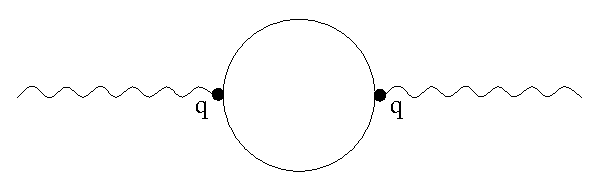
\epsfig{file=fig.eps,height=1in}}


\vskip.35in



Clearly, this diagram gives a multiplicative factor of $q^2$.
It also diverges logarithmically for $u\mapsto u_0$.
The result is that for $u$ near $u_0$ we have:
$$\tau(u)=2q^2\frac{{\rm ln}(u-u_0)+{\rm constant}}{2\pi i}.$$
This means that the monodromy of $\tau(u)$ in $PSL_2({\bf Z})$ around this
singularity is 
\begin{equation}\label{qformula}
\pm \pmatrix{ 1 & 2q^2 \cr 0 & 1}.
\end{equation}

Of course, the monodromy is actually an element in $SL_2({\bf Z})$ and
is only 
determined up to sign by the monodromy in $PSL_2({\bf Z})$
To pin down the sign we argue as follows.
The physics near $u=u_0$ is described by a $U(1)$-gauge theory with
gauge fields $(\tilde A,\tilde a)$ and a charged hyper-multiplet $(T,T')$
which is becoming massless at $u_0$.
Thus, the Lagrangian is of the form of the gauge couplings plus a
super-potential $\tilde aqTT'$.  
The scalar field $\tilde a$ is a local coordinate on the $u$-plane and
in fact is related to $a,a_D$ at infinity by an $ISL_2({\bf Z})$
transformation.  (The image of this transformation in $SL_2({\bf Z})$
is determined by the charge 
$(n_e,n_m)$ of the hyper-multiplet $(T,T')$ with respect to the $U(1)$
at infinity in the $u$-plane.)
 Since the $U(1)$-theory exists throughout this
neighborhood even at the singularity,
we see that under monodromy around $u_0$
the field $\tilde a$ comes back to itself.
This implies that there is an invariant vector under the $SL_2({\bf
Z})$-monodromy around $u_0$ and hence shows that the monodromy is as
written in Equation~\ref{qformula} with a plus sign.







We can generalize this picture. Suppose that at $u_0$ there are
several hyper-multiplets of charge $q_i$ becoming massless. Then the
local form of $\tau$ would be
$$\tau = 2\sum_iq_i^2 \frac{{\rm ln}(u-u_0)+{\rm constant}}{2\pi i}$$
and the 
monodromy around $u_0$ would be 
$$\pmatrix{1 & \sum_i2q^2_i \cr 0 & 1}.$$


Notice that the monodromy around a singularity where a hyper-multiplet
is becoming massless has trace $2$ whereas the monodromy at infinity
has trace $-2$.
This means in particular, that there cannot be only one singularity in
the $u$-plane if the singularity is of this type.
(This of course also follows from the positivity of $\tau$ in the
complement of the singularities.)

\subsection{The number of singularities in ${\cal M}$}




To understand the number of singularities in ${\cal M}$, let us begin
with a microscopic $N=2$ super-symmetric $SU(2)$-theory and
break it to 
an $N=1$ super-symmetric theory by adding a perturbation of the form
\begin{equation}\label{pert}
\Delta{\cal L}=\int d^4xd^2\theta mu +{\rm c.c},
\end{equation}
with $m$ a complex constant.
(Recall that $u={\rm Tr}\phi^2$.)
This theory has two vacua, each with a mass gap and with confinement.

Let us suppose that at a point in the space of quantum vacua we have
$N_h$ hyper-multiplets becoming 
massless, say $(T_i,T'_i)$ of charge $q_i$.
So near this point the physics is described by a super potential
$$W=\tilde a\left(\sum_iq_iT_iT_i'\right) +mu(\tilde a).$$
where, as before $\tilde a$ is a local parameter on the $u$-plane and
is related by an $SL_2({\bf Z})$ transformation to $a,a_D$ at
infinity. 
Let us find the space of  vacua in the macroscopic theory.  That is to
say we solve $dW=0$ and divide by the ${\bf C}^*$-action.  Clearly,
the equation $dW=0$  is equivalent to
$$\tilde aT_i=\tilde aT_i'=0\ \ \ {\rm  for\  all\ \ }i.$$
$$m\frac{du}{d\tilde a}+\sum_Iq_iT_iT'_i=0.$$
If $N_h>0$ this gives us a positive dimensional space of vacua. This
is impossible since the microscopic theory has only two vacua.
This means that (as indicated above) at each singularity we have only
one hyper-multiplet 
becoming massless.
Furthermore, since $\frac{du}{d\tilde a}\not= 0$ we see
from the second equation that $T,T'\not=0$.  By the first equation,
this means that $\tilde a=0$.
Since there is only one hyper-multiplet, the equation becomes
$$m\frac{du}{d\tilde a}|_{\tilde a=0}
+qTT'=0.$$
This determines the vacuum uniquely up to the action of ${\bf
C}^*$. Thus, we see that there is a unique vacuum associated to this
singularity. 
Having one vacuum for each singularity
in the macroscopic theory, and having only two vacua in the
microscopic theory, it follows that there are at most two
singularities in ${\cal M}$. Notice also that the critical points for
$u$ on ${\cal M}$ also give vacua in the macroscopic theory.  Thus, we see
$$N_c+N_h\le 2$$
where $N_c$ is the number of critical points in ${\cal M}$ of the
analytic function $u$ and $N_h$ is the number of points at which a
hyper-multiplet becomes massless.


As we have already remarked, the monodromy around a point where a
hyper-multiplet is massless and the monodromy at infinity have opposite
traces and hence are not conjugate in $SL_2({\bf Z})$.
At a critical point of $u$ there is no monodromy.
Thus, these facts about monodromy imply that  $N_h\ge 2$. 
It follows that $N_h=2$ and $N_c=0$. That is to say $u\colon {\cal
M}\to {\bf C}$ is everywhere a local analytic isomorphism.  Since it
is an isomorphism between neighborhoods of infinity, it follows that
$u\colon {\cal M}\to {\bf C}$ is an isomorphism.
(Recall that we established this fact directly from the fact that $u$
is an isomorphism at infinity. This gives a consistency check on our
model.) 
Even though the spaces of classical and quantum vacua are identified,
there are important differences.
Whereas classically, there is only one singular point in the $u$-plane
and at this singular point the $SU(2)$-theory is restored as the low
energy limit, quantum
mechanically there are 
two singularities in the $u$-plane (at as yet to be identified
points), and at each of these a charged 
spin $1/2$ hyper-multiplet  becomes massless. Furthermore, unlike the
classical case, the monodromy in the quantum family is non-trivial in
$PSL_2({\bf Z})$.  This implies that, unlike the classical case, the
family of tori over the 
space of quantum vacua do not have constant $j$-invariant.


Notice that now that we have found two singularities in the $u$-plane,
each contributing a vacuum when we add the perturbation in
Equation~\ref{pert}.  Since there are at most two vacua in the
perturbed theory, it follows that there cannot be isolated points of
the space of quantum vacua; these
isolated points would also  produce quantum vacua of the perturbed
theory. 


The $U(1)_R$-symmetry is broken down to a ${\bf Z}/8{\bf Z}$-symmetry
which since $u$ has charge four under $U(1)_R$ acts on the $u$-plane
as a ${\bf Z}/2{\bf Z}$-symmetry. It is the symmetry $u\mapsto -u$. 
This implies
that the two singularities in ${\cal M}$ are at points $\pm u_0$ for
some $u_0\not= 0$. As we have already seen dimensional analysis tells
us that $u$ goes like $\Lambda^2$, the square of the mass parameter in
the theory. This means that we can make a choice of the mass
parameter  $\Lambda$ so that  
the quantum theory labeled by  $\Lambda$ has singularities at
$u=\pm \Lambda^2$. In this way we are adopting the precise definition of
the mass scale parameter $\Lambda$  promised in the introduction.
Notice that this  choice of $\Lambda$ is different from the one that
we have used until now.  The only affect of this change in the choice of
$\Lambda$ simply is to introduce an additive constant into
Formulas~\ref{tau1} through~\ref{tau4}. 

\subsection{The new massless particles}

The next step is to identify what is becoming massless.
Let $(n_e,n_m)$  be the charge of the  hyper-multiplet
becoming massless at $\Lambda^2$ when we express things in the basis
in which the monodromy at infinity is upper 
triangular. If $n_m=0$, then the monodromy at $\Lambda^2$ commutes
with the monodromy at infinity.  Since the total space of the
non-singular part of the family is the three-times punctured sphere,
the monodromies at $\Lambda^2$ and $\infty$ generate the entire monodromy
image. Thus, if the monodromy at $\infty$ and $\Lambda^2$ are
simultaneously upper triangular, then the entire monodromy image is
upper triangular and hence commutative.
This would mean that ${\rm Im}\tau$ could not be positive everywhere.
Our conclusion is that $n_m\not=0$.  That is to
say, the particle becoming massless at $u=\Lambda^2$ is magnetically
charged. 
Exactly the same analysis holds for the singularity at $-\Lambda^2$.
This is a very interesting phenomenon.  Particles which started life
when $|u|>>\Lambda^2$ as massive solitons are becoming massless as $u$
approaches $\pm \Lambda^2$.
Also, it means that our description of the theory near $\pm \Lambda^2$
as a $U(1)$-theory is a different representation from the
$U(1)$-representation of the theory near infinity in the $u$-plane.


Now we wish to calculate the magnetic charge $\pm n_m$ of these particles.
Notice that as we come in from infinity $\pm n_m$ is well-defined
independent of the path we choose from infinity to $\pm \Lambda^2$ but
the electric charge depends on the path -- if we wind around the pair
of singularities $\pm n_e$ changes by twice the magnetic charge, since
the monodromy around infinity is $n_e\mapsto -n_e+2n_m$. 



The model we are discussing today has various mathematical applications,
but just in terms of physics one of its most striking applications
was to give a new model of confinement.  We recall that confinement is
the statement that there is a 
linear potential between  external electric charges or alternatively
that there is  area
law decay for a Wilson loop in the  an appropriate representation
(in the present example, the two-dimensional representation of $SU(2)$).
We recall that in  a Higgs phase, where a charged field gets a vacuum
expectation value\footnote{This is a somewhat imprecise description as we have
seen in previous lectures, but is valid in weak  coupling.}, one can
explicitly calculate by a topological argument that the 't Hooft loop
gets area law decay.  If one could just naively exchange electricity and
magnetism, then Wilson loops would be exchanged with 't Hooft loops
and we would conclude  that confinement will arise if a magnetically
charged field gets a vacuum expectation value.  This was
argued heuristically in the 1970's by 't Hooft,
Mandelstam, Nambu and others but with great difficulty in exhibiting
actual models, since usually one does not have magnetically charged
fields in the formalism 
and magnetically charged objects (which arise as classical solutions)
are heavy in the weakly
coupled regime where one understands them concretely.  Thus it was generally
rather hard to see how one could actually exhibit a phenomenon in which
a magnetically charged field gets a vacuum expectation value.



In the present context, this happens.  We have already seen
that after adding the $mu$ perturbation to the superpotential, which
is expected to give confinement,
 the vacuum near $u=\Lambda^2$ has $T,T'\not=0$, so in fact in this
vacuum ($n_m$ being non-zero) a magnetically charged object has obtained
a vacuum expectation value.  Thus as expected a magnetically charged
field obtained a vacuum expectation value just in the confining case.
(To pursue this with greater precision, it is important that the magnetically
charged field in question has $n_m$ odd.  Indeed, as the center of $SU(2)$
is ${\bf Z}/2{\bf Z}$, the explanation of confinement via a dual of the usual
Higgs mechanism requires a nonzero expectation value of a field of
odd $n_m$.  We will see that $n_m$ actually is odd, in fact $\pm 1$,
for $T$ and $T'$.)  



Notice something surprising has happened.  The magnetic monopoles have
mass at infinity  on the order of $\sqrt{|u|}{\rm ln}(|u|)$ whereas
there are other BPS states of masses on the order of
$\sqrt{|u|}$. Thus, at infinity the monopoles are not the least
massive of the massive particles.  Nevertheless, they are the ones
becoming massless at the singular points.


\subsection{Explicit nature of the family of elliptic curves}

We are now ready to describe the macroscopic theory associated to the
quantum theory labeled by mass parameter $\Lambda$ by describing
explicitly the family of elliptic curves and the two-form $\eta$
associated with the space of quantum vacua of this theory.
As we have seen, for this theory  the
moduli space of quantum vacua is ${\bf C}$ with 
parameter $u={\rm Tr}\phi^2$. The $SL_2({\bf Z})$-monodromy at
infinity for the family is 
$$\pmatrix{-1 & 2 \cr 0 & -1}.$$
There are in addition two other points $\pm\Lambda^2$ in the $u$-plane
where there are singularities.  The $SL_2({\bf Z})$-monodromy,
$m_{\pm\Lambda^2}$   at each of these points has trace two.
We write 
$$m_{\Lambda^2}^{-1}=\pmatrix{1+b & -b^2/a \cr a & 1-b},$$
for integers $a,b$.
(This is the general form of a matrix of trace two and determinant one.)
Since
$$m_{-\Lambda^2}=m_{\Lambda^2}^{-1}m_\infty$$
has trace two, 
we conclude that
$$2={\rm Tr}\pmatrix{1+b & -b^2/a \cr a & 1-b}\pmatrix{-1 & 2 \cr 0 &
-1}.$$ 

It follows by a direct computation that $a=2$.
Since $-b^2/a$ is an integer, we see that $b$ is even.
Now let us conjugate the matrix for $m_{\Lambda^2}^{-1}$ by the matrix 
$$\pmatrix{1 & 1 \cr 0 & 1},$$
which commutes with the monodromy at infinity.
The result is to change $b$ by $2$. Thus, after a number of these
conjugations we arrive at $b=0$.
This means that in an appropriate basis the monodromy at infinity is
$$\pmatrix{ -1 & 2 \cr 0 & -1}$$
 and the monodromy at $\Lambda^2$ is of the form
$$\pmatrix{1 & 0 \cr -2 & 1}.$$
Thus, we have shown that the monodromy  representation is uniquely
determined up to conjugation in $SL_2({\bf Z})$. 
Notice also that according to Equation~\ref{qformula} the magnetic
charge $n_m$ of the hyper-multiplet that is becoming masses at
$\Lambda^2$ is $\pm 1$.  The same of course holds at $-\Lambda^2$. 
In fact, because the $SL_2({\bf Z})$ is uniquely determined up to
conjugation it is invariant, up to conjugation, under the symmetry
$u\mapsto -u$. 

It is easy to identify the family of elliptic curves over the twice
punctured plane with this monodromy.  The base of the family can be
identified with
the modular curve ${\bf H}/\Gamma(2)$ given by dividing
out the upper half-plane by the (free) action of the subgroup of
$PSL_2({\bf Z})$ consisting of all matrices congruent to the identity
modulo two.
The family  is the universal family of
elliptic curves with `level two structure' over this base.
Since the singularities 
are at $u=\pm\Lambda^2$, the Weierstrass equation for the
family of elliptic curves associated to this quantum theory is 
$$y^2=(x-u)(x-\Lambda^2)(x+\Lambda^2).$$




Now let us consider the  two-form $\eta$ as described in the last
lecture. We know that in the Weierstrass model given above $\eta$ has
the general form 
$$\eta=f(u)du\frac{dx}{y}.$$
Implicitly in the discussions before we assumed that $\eta$ was a
complex symplectic form without zeros or poles at least away from the
exceptional values of $u$. Such zeros or poles
would produce non-physical singularities.
If we take $f$ to be a non-zero constant, then the K\"ahler form
$\pi_*(\eta\wedge \overline\eta)$ is smooth except at $\infty,\pm
\Lambda^2$ where it has the correct singular behavior.  Any other $f$ would
produce either poles or zeros at other points or the wrong singular
behavior at one of $\infty,\pm\Lambda^2$.
It follows that $\eta=Cdu\frac{dx}{y}$ for an appropriate constant
which can be computed by comparing to the formula $a^2=u$ near
$u=\infty$. 

Clearly,
$$\eta=d\left(C\frac{udx}{y}\right)=
d\left(C\frac{2ydx}{x^2-\Lambda^4}\right).$$ 

The form $\lambda=2Cydx/(x^2-\Lambda^4)$
is a differential of the second 
kind on the total space ${\cal E}$ of the family of elliptic curves.
This means, as we have been asserting all along, that $[\eta]\in
H^2({\cal E};{\bf C})$ is trivial and hence that 
the monodromy of
our family of representations of the theory is contained in $SL_2({\bf
Z})$, inside the bigger group $ISL_2({\bf Z})$. This was expected
since  the theory has no  conserved charges except $n_e,n_m$. 

\subsection{Description of the BPS spectrum}

The line in the $u$-plane where $a/a_D$ is real is a simple closed
curve that passes through the points $u=\pm\Lambda^2$. 
The spectrum of BPS states is continuous off this circle.
Approaching from $u=\infty$, we see that 
 at $u=\Lambda^2$ we have $a=0$ and $a_D\not= 0$, whereas at
$u=-\Lambda^2$ we have $-a+a_D=0$. (Of course, the exact values depend
on the path chosen from $\infty$ to $\pm\Lambda^2$, but if we come in
along rays from infinity toward the origin then given equations hold.)
Since we can approach the two singularities from infinity without
crossing the jumping locus for the BPS states, we see that the BPS
states that are becoming massless at $u=\pm\Lambda^2$ are indeed among
the original BPS states at infinity.  That is to say, these particles
are analytic continuations of the original magnetic monopoles at
infinity. 

Now let us examine whether, at other points on the jumping locus
besides $\pm\Lambda^2$, there are particles forced to become
massless. As we move along the jumping line on the open upper arc from
$\Lambda^2$ to 
$-\Lambda^2$, we find that for
every $s, 0 < s <1$ there is a point where
$sa-a_D=0$.
So if  there is a BPS state at infinity has charges $(n_e,n_m)$ with 
$(n_e,n_m)=t(s,-1)$ for some $t\in {\bf R}$, then at some point along
this open arc we find that this state becomes massless.
This, and the symmetric argument for
the open lower arc of the jumping line, show that all the BPS states
at infinity that satisfy 
$$(n_e,n_m)=(p,\pm q)$$
with $0<p<q$ become massless somewhere on the jumping curve  minus
$\pm\Lambda^2$. 
But  we know by our analysis of the singularities that there
are no points on these open arcs where BPS states (or any other
charged states) become massless.  The conclusion is that there are no
BPS states at infinity satisfying the above inequality. Said another
way the only BPS states at infinity are those of charges
$$(n_e,n_m)=(\pm 1,0)$$
$$(n_e,n_m)=(p,\pm 1).$$
Of course, these are exactly the BPS states that do exist at infinity.
The first are the vector multiplets and the second are the magnetic
monopoles. 
This gives us a check of the internal consistency of the theory.

This analysis of the BPS  spectrum in the quantum theory can be
compared in an interesting way to the following classical 
computation.  Let ${\cal M}_k$ be the moduli space of $k$-monopole
solutions of this theory, reduced by dividing by translations.  It is
a hyperk\"ahler manifold of dimension $4k-4$ that has been much
studied mathematically.  It can be shown that $L^2$-holomorphic forms
(possibly valued in a flat line bundle) on ${\cal M}_k$ would give
$k$-monopole bound states, for $k>1$.  From what we have seen, there
should be no such bound states, so there should be no $L^2$-holomorphic
forms on ${\cal M}_k$.  More generally, an argument by Sen using
duality of $N=4$ super Yang-Mills (rather than the $N=2$ theory that
we have considered in this lecture) determines the full
$L^2$-cohomology of the ${\cal M}_k$.

\end{document}







